\documentclass{ds201}

% =============================================
% Part 0 信息
% =============================================

\mathsetup{
  % 学生姓名
  student-name = {某同学},
  % 学号
  student-id = {2022****},
  % 班级
  student-class = {2022121},
  % 指导老师
  teacher = {竺筱晶},
  % 日期——年
  year = {2023},
  % 日期——月
  month = {12},
  % 日期——日
  day= {1},
}

\begin{document}

% =============================================
% Part 1  封面
% =============================================

\makecover

% \tableofcontents

% \newpage 

% =============================================
% Part 2 主文档
% =============================================

\section{最大流在工作指派问题中的应用}

考虑工作指派问题的线性规划模型:

$min\ T$

s.t.\ \ $\sum_{j \in S_i} x_{ij} =t_i,  i\in\text{\textbraceleft}1,...,n\text{\textbraceright}$

\ \ \ \ \ \ $\sum_{i:j \in S_i} x_{ij}<=T,  j\in\text{\textbraceleft}1,...,m\text{\textbraceright}$

\ \ \ \ \ \ $x_{ij}>0, i\in\text{\textbraceleft}1,...,n\text{\textbraceright},j\in S_i$

用课件中介绍的最大流模型求解该问题,具体采用如下二分搜索算法:

step1:设$T_1=0$,$T_u$是一个充分大的数

step2:令$T=0.5*(T_l+T_u)$

step3:如果最大流的值为$\sum_{i=1}^n t_i$,则令$T_u=T$。

\ \ \ \ \ \ \ \ \ \ 如果最大流的值小于$\sum_{i=1}^n t_i$,则令$T_l=T$。

step4:回到step2

请编写上述算法的Matlab或Python程序,其中Step2的最大流算法可以用Matlab或Python自带函数也可以自己编程(用自带函数满分只有90分),并用数值例子检验程序。在数值例子中,
取n=9,m=5,各项工作的处理时间分别为$t_1=3$、$t_2=3$、$t_3=4$、$t_4=4$、$t_5=5$、$t_6=5$、$t_7=6$、$t_8=10$、$t_9=13$,各项工作的工人集分别为
$S_1=\text{\textbraceleft}1,2\text{\textbraceright}$、$S_2=\text{\textbraceleft}1,3\text{\textbraceright}$、
$S_3=\text{\textbraceleft}2,5\text{\textbraceright}$、$S_4=\text{\textbraceleft}1,4\text{\textbraceright}$、
$S_5=\text{\textbraceleft}2,5\text{\textbraceright}$、$S_6=\text{\textbraceleft}4,5\text{\textbraceright}$、
$S_7=\text{\textbraceleft}3,5\text{\textbraceright}$、$S_8=\text{\textbraceleft}3,4\text{\textbraceright}$、
$S_9=\text{\textbraceleft}3,4\text{\textbraceright}$。
\subsection{解题思路}

\subsection{数值结果}
\begin{figure}[H]
  \centering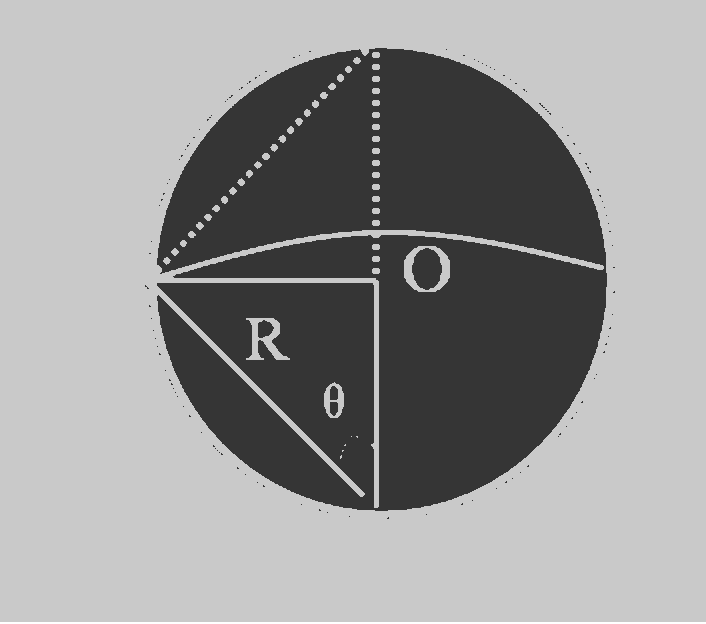
\includegraphics[width=0.3\linewidth]{01.png}
  \label{img01}
\end{figure}

\subsection{程序代码}

\inputminted[
    frame=lines,
    framesep=2mm,
    baselinestretch=1.2,
    fontsize=\small,
    linenos
]{python}{code/lab01.py}

\section{感想和体会}

\section{个人申明}

\end{document}
